

\tikzset{every picture/.style={line width=0.3pt}} %set default line width to 0.75pt        

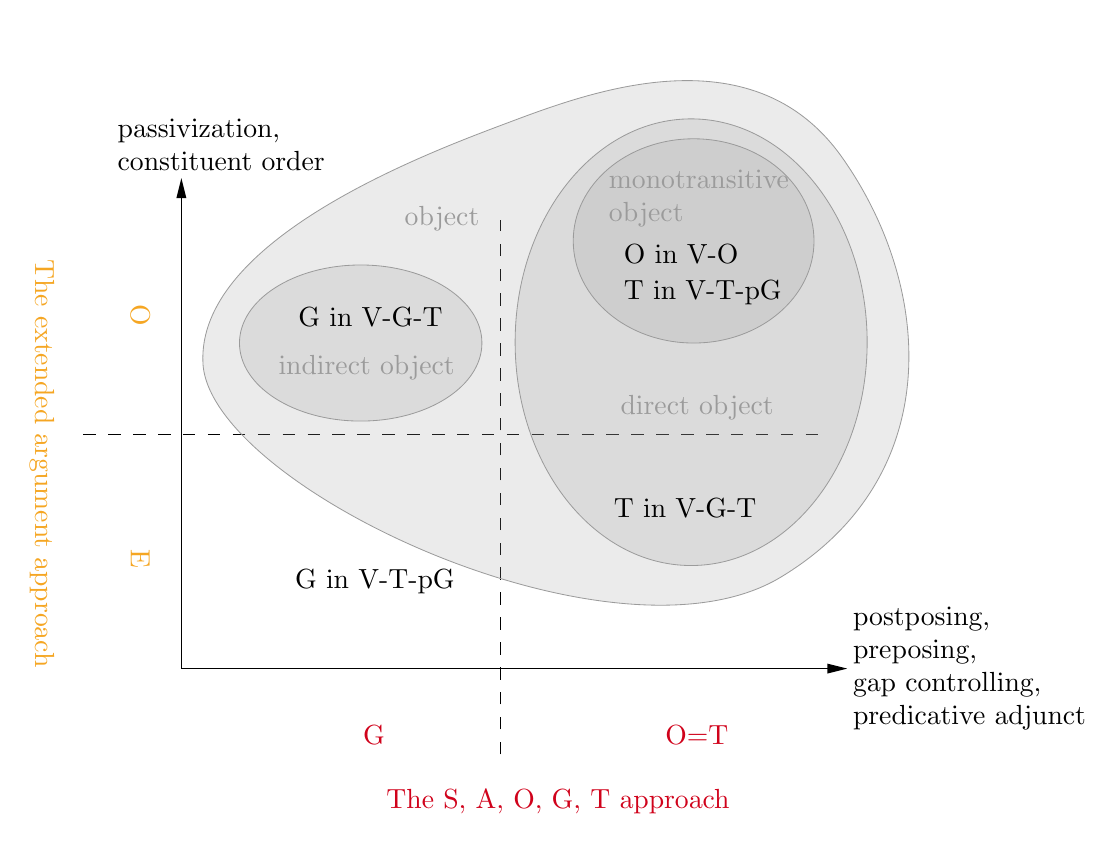
\begin{tikzpicture}[x=0.75pt,y=0.75pt,yscale=-0.8,xscale=0.8]
%uncomment if require: \path (0,500); %set diagram left start at 0, and has height of 500

%Straight Lines [id:da5593585477377434] 
\draw    (107,391) -- (506,391) ;
\draw [shift={(508,391)}, rotate = 180] [fill={rgb, 255:red, 0; green, 0; blue, 0 }  ][line width=0.08]  [draw opacity=0] (12,-3) -- (0,0) -- (12,3) -- cycle    ;
%Straight Lines [id:da7245999585667466] 
\draw    (107,391) -- (107,97.59) ;
\draw [shift={(107,95.59)}, rotate = 90] [fill={rgb, 255:red, 0; green, 0; blue, 0 }  ][line width=0.08]  [draw opacity=0] (12,-3) -- (0,0) -- (12,3) -- cycle    ;
%Straight Lines [id:da8964896003323979] 
\draw  [dash pattern={on 4.5pt off 4.5pt}]  (48,250) -- (494,250) ;
%Straight Lines [id:da9625166392954305] 
\draw  [dash pattern={on 4.5pt off 4.5pt}]  (299,442.59) -- (299,120.59) ;
%Shape: Ellipse [id:dp7384360040390137] 
\draw  [color={rgb, 255:red, 155; green, 155; blue, 155 }  ,draw opacity=1 ][fill={rgb, 255:red, 155; green, 155; blue, 155 }  ,fill opacity=0.2 ] (343,133.43) .. controls (343,99.46) and (375.46,71.93) .. (415.5,71.93) .. controls (455.54,71.93) and (488,99.46) .. (488,133.43) .. controls (488,167.39) and (455.54,194.93) .. (415.5,194.93) .. controls (375.46,194.93) and (343,167.39) .. (343,133.43) -- cycle ;
%Shape: Ellipse [id:dp035938837693224146] 
\draw  [color={rgb, 255:red, 155; green, 155; blue, 155 }  ,draw opacity=1 ][fill={rgb, 255:red, 155; green, 155; blue, 155 }  ,fill opacity=0.2 ] (308,194.43) .. controls (308,120.14) and (355.46,59.93) .. (414,59.93) .. controls (472.54,59.93) and (520,120.14) .. (520,194.43) .. controls (520,268.71) and (472.54,328.93) .. (414,328.93) .. controls (355.46,328.93) and (308,268.71) .. (308,194.43) -- cycle ;
%Shape: Ellipse [id:dp04989243684342659] 
\draw  [color={rgb, 255:red, 155; green, 155; blue, 155 }  ,draw opacity=1 ][fill={rgb, 255:red, 155; green, 155; blue, 155 }  ,fill opacity=0.2 ] (142,194.93) .. controls (142,168.97) and (174.68,147.93) .. (215,147.93) .. controls (255.32,147.93) and (288,168.97) .. (288,194.93) .. controls (288,220.88) and (255.32,241.93) .. (215,241.93) .. controls (174.68,241.93) and (142,220.88) .. (142,194.93) -- cycle ;
%Shape: Polygon Curved [id:ds6446496039380643] 
\draw  [color={rgb, 255:red, 155; green, 155; blue, 155 }  ,draw opacity=1 ][fill={rgb, 255:red, 155; green, 155; blue, 155 }  ,fill opacity=0.2 ] (301,63.26) .. controls (349,45.26) and (450,5.26) .. (505,83.26) .. controls (560,161.26) and (568,275.59) .. (468,335.93) .. controls (368,396.26) and (124,281.26) .. (120,207.26) .. controls (116,133.26) and (253,81.26) .. (301,63.26) -- cycle ;

% Text Node
\draw (131,92.59) node [anchor=south] [inner sep=0.75pt]   [align=left] {passivization,\\constituent order};
% Text Node
\draw (510,391) node [anchor=west] [inner sep=0.75pt]   [align=left] {postposing,\\preposing,\\gap controlling,\\predicative adjunct};
% Text Node
\draw (176,172) node [anchor=north west][inner sep=0.75pt]   [align=left] {G in V-G-T};
% Text Node
\draw (174,330) node [anchor=north west][inner sep=0.75pt]   [align=left] {G in V-T-pG};
% Text Node
\draw (372,134) node [anchor=north west][inner sep=0.75pt]   [align=left] {O in V-O};
% Text Node
\draw (372,156) node [anchor=north west][inner sep=0.75pt]   [align=left] {T in V-T-pG};
% Text Node
\draw (366,287) node [anchor=north west][inner sep=0.75pt]   [align=left] {T in V-G-T};
% Text Node
\draw (215,424) node [anchor=north west][inner sep=0.75pt]  [color={rgb, 255:red, 208; green, 2; blue, 27 }  ,opacity=1 ] [align=left] {G};
% Text Node
\draw (397,424) node [anchor=north west][inner sep=0.75pt]  [color={rgb, 255:red, 208; green, 2; blue, 27 }  ,opacity=1 ] [align=left] {O=T};
% Text Node
\draw (89.5,170.5) node [anchor=north west][inner sep=0.75pt]  [color={rgb, 255:red, 245; green, 166; blue, 35 }  ,opacity=1 ,rotate=-90] [align=left] {O};
% Text Node
\draw (89.5,317.5) node [anchor=north west][inner sep=0.75pt]  [color={rgb, 255:red, 245; green, 166; blue, 35 }  ,opacity=1 ,rotate=-90] [align=left] {E};
% Text Node
\draw (32,143) node [anchor=north west][inner sep=0.75pt]  [color={rgb, 255:red, 245; green, 166; blue, 35 }  ,opacity=1 ,rotate=-90] [align=left] {The extended argument approach};
% Text Node
\draw (229,462) node [anchor=north west][inner sep=0.75pt]  [color={rgb, 255:red, 208; green, 2; blue, 27 }  ,opacity=1 ] [align=left] {The S, A, O, G, T approach};
% Text Node
\draw (363,89) node [anchor=north west][inner sep=0.75pt]  [color={rgb, 255:red, 155; green, 155; blue, 155 }  ,opacity=1 ] [align=left] {monotransitive \\object};
% Text Node
\draw (370,225) node [anchor=north west][inner sep=0.75pt]  [color={rgb, 255:red, 155; green, 155; blue, 155 }  ,opacity=1 ] [align=left] {direct object};
% Text Node
\draw (164,201) node [anchor=north west][inner sep=0.75pt]  [color={rgb, 255:red, 155; green, 155; blue, 155 }  ,opacity=1 ] [align=left] {indirect object};
% Text Node
\draw (240,111) node [anchor=north west][inner sep=0.75pt]  [color={rgb, 255:red, 155; green, 155; blue, 155 }  ,opacity=1 ] [align=left] {object};


\end{tikzpicture}
